%%%%%%%%%%%%%%%%%%%%%%%%%%%%%%%%%%%%%%%%%
% Arsclassica Article
% LaTeX Template
% Version 1.1 (1/8/17)
%
% This template has been downloaded from:
% http://www.LaTeXTemplates.com
%
% Original author:
% Lorenzo Pantieri (http://www.lorenzopantieri.net) with extensive modifications by:
% Vel (vel@latextemplates.com)
%
% License:
% CC BY-NC-SA 3.0 (http://creativecommons.org/licenses/by-nc-sa/3.0/)
%
%%%%%%%%%%%%%%%%%%%%%%%%%%%%%%%%%%%%%%%%%

%----------------------------------------------------------------------------------------
%	PACKAGES AND OTHER DOCUMENT CONFIGURATIONS
%----------------------------------------------------------------------------------------

\documentclass[
10pt, % Main document font size
a4paper, % Paper type, use 'letterpaper' for US Letter paper
oneside, % One page layout (no page indentation)
%twoside, % Two page layout (page indentation for binding and different headers)
headinclude,footinclude, % Extra spacing for the header and footer
BCOR5mm, % Binding correction
]{scrartcl}

%%%%%%%%%%%%%%%%%%%%%%%%%%%%%%%%%%%%%%%%%
% Arsclassica Article
% Structure Specification File
%
% This file has been downloaded from:
% http://www.LaTeXTemplates.com
%
% Original author:
% Lorenzo Pantieri (http://www.lorenzopantieri.net) with extensive modifications by:
% Vel (vel@latextemplates.com)
%
% License:
% CC BY-NC-SA 3.0 (http://creativecommons.org/licenses/by-nc-sa/3.0/)
%
%%%%%%%%%%%%%%%%%%%%%%%%%%%%%%%%%%%%%%%%%

%----------------------------------------------------------------------------------------
%	REQUIRED PACKAGES
%----------------------------------------------------------------------------------------

\usepackage[
nochapters, % Turn off chapters since this is an article        
beramono, % Use the Bera Mono font for monospaced text (\texttt)
eulermath,% Use the Euler font for mathematics
pdfspacing, % Makes use of pdftex’ letter spacing capabilities via the microtype package
dottedtoc % Dotted lines leading to the page numbers in the table of contents
]{classicthesis} % The layout is based on the Classic Thesis style

\usepackage{arsclassica} % Modifies the Classic Thesis package

\usepackage{float}

\usepackage[T1]{fontenc} % Use 8-bit encoding that has 256 glyphs

\usepackage[utf8]{inputenc} % Required for including letters with accents

\usepackage{graphicx} % Required for including images
\graphicspath{{Figures/}} % Set the default folder for images

\usepackage{enumitem} % Required for manipulating the whitespace between and within lists

\usepackage{lipsum} % Used for inserting dummy 'Lorem ipsum' text into the template

\usepackage{subfig} % Required for creating figures with multiple parts (subfigures)

\usepackage{amsmath,amssymb,amsthm} % For including math equations, theorems, symbols, etc

\usepackage{varioref} % More descriptive referencing

%----------------------------------------------------------------------------------------
%	THEOREM STYLES
%---------------------------------------------------------------------------------------

\theoremstyle{definition} % Define theorem styles here based on the definition style (used for definitions and examples)
\newtheorem{definition}{Definition}

\theoremstyle{plain} % Define theorem styles here based on the plain style (used for theorems, lemmas, propositions)
\newtheorem{theorem}{Theorem}

\theoremstyle{remark} % Define theorem styles here based on the remark style (used for remarks and notes)

%----------------------------------------------------------------------------------------
%	HYPERLINKS
%---------------------------------------------------------------------------------------

\hypersetup{
%draft, % Uncomment to remove all links (useful for printing in black and white)
colorlinks=true, breaklinks=true, bookmarks=true,bookmarksnumbered,
urlcolor=webbrown, linkcolor=RoyalBlue, citecolor=webgreen, % Link colors
pdftitle={}, % PDF title
pdfauthor={\textcopyright}, % PDF Author
pdfsubject={}, % PDF Subject
pdfkeywords={}, % PDF Keywords
pdfcreator={pdfLaTeX}, % PDF Creator
pdfproducer={LaTeX with hyperref and ClassicThesis} % PDF producer
} % Include the structure.tex file which specified the document structure and layout

\hyphenation{Fortran hy-phen-ation} % Specify custom hyphenation points in words with dashes where you would like hyphenation to occur, or alternatively, don't put any dashes in a word to stop hyphenation altogether
\usepackage{stix} % Use the STIX fonts

%----------------------------------------------------------------------------------------
%	TITLE AND AUTHOR(S)
%----------------------------------------------------------------------------------------

\title{\normalfont\spacedallcaps{Operations Manual}} % The article title

%\subtitle{Subtitle} % Uncomment to display a subtitle

\author{\spacedlowsmallcaps{Samantha Freitas \& Adrian Beehner*}} % The article author(s) - author affiliations need to be specified in the AUTHOR AFFILIATIONS block

\date{} % An optional date to appear under the author(s)

%----------------------------------------------------------------------------------------

\begin{document}

%----------------------------------------------------------------------------------------
%	HEADERS
%----------------------------------------------------------------------------------------

\renewcommand{\sectionmark}[1]{\markright{\spacedlowsmallcaps{#1}}} % The header for all pages (oneside) or for even pages (twoside)
%\renewcommand{\subsectionmark}[1]{\markright{\thesubsection~#1}} % Uncomment when using the twoside option - this modifies the header on odd pages
\lehead{\mbox{\llap{\small\thepage\kern1em\color{halfgray} \vline}\color{halfgray}\hspace{0.5em}\rightmark\hfil}} % The header style

\pagestyle{scrheadings} % Enable the headers specified in this block

%----------------------------------------------------------------------------------------
%	TABLE OF CONTENTS & LISTS OF FIGURES AND TABLES
%----------------------------------------------------------------------------------------

\maketitle % Print the title/author/date block

\setcounter{tocdepth}{2} % Set the depth of the table of contents to show sections and subsections only

\tableofcontents % Print the table of contents


%----------------------------------------------------------------------------------------
%	AUTHOR AFFILIATIONS
%----------------------------------------------------------------------------------------

\let\thefootnote\relax\footnotetext{* \textit{Research Head, Idaho Catfish Project, Coeur d'Alene, Idaho}}

%----------------------------------------------------------------------------------------

\newpage % Start the article content on the second page, remove this if you have a longer abstract that goes onto the second page

%----------------------------------------------------------------------------------------
%	INTRODUCTION
%----------------------------------------------------------------------------------------

\section{Introduction}
\subsection*{Overview}

Northern Idaho is one of the regions in the western United States that has seen extensive mining operations. The South fork of the Coeur d’Alene river has carried heavy metal contaminated sediments from silver and lead mining to the Coeur d’Alene lakebed. By developing an underwater drone capable of descending to deep-water, we become able to read the water quality in lakes and reservoirs. This will allow better supervision of water bodies and management of toxicity.

\subsection*{Purpose \& Scope}

This project focuses on creating and/or beginning development of an autonomous submarine that will collect water quality data in deep-water lakes and reservoirs. This submarine, dubbed the “Idaho Catfish”, will be able to perform such underwater surveys by continuously sampling a variety of water quality variables such as oxygen, pH, temperature, etc. The end result will be that the Catfish will be fully autonomous, but tethered instructions will also be provided.

\subsection*{Term Definitions?}

\textit{Idaho Catfish }  – The submarine nickname. \\ \\
\textit{Tethered } – The wires that connect the submarine to the surface, allowing for direct control and easier tracking of the submarine. Currently the submarine only runs tethered, it is not fully autonomous. \\ \\
\textit{ V } - Stands for voltage, a way of measuring a charge in batteries. \\ \\
\textit{Handling Gear} - The set of gear that aids in deploying the submarine. Contains the tether, a winch, battery, communications module, and various storage. See Diagram \\ \\

\newpage
 
%----------------------------------------------------------------------------------------
%	BASIC OPS
%----------------------------------------------------------------------------------------

\section{Basic Operations}
\subsection{Components}
\begin{figure}[H]
	\centering 
	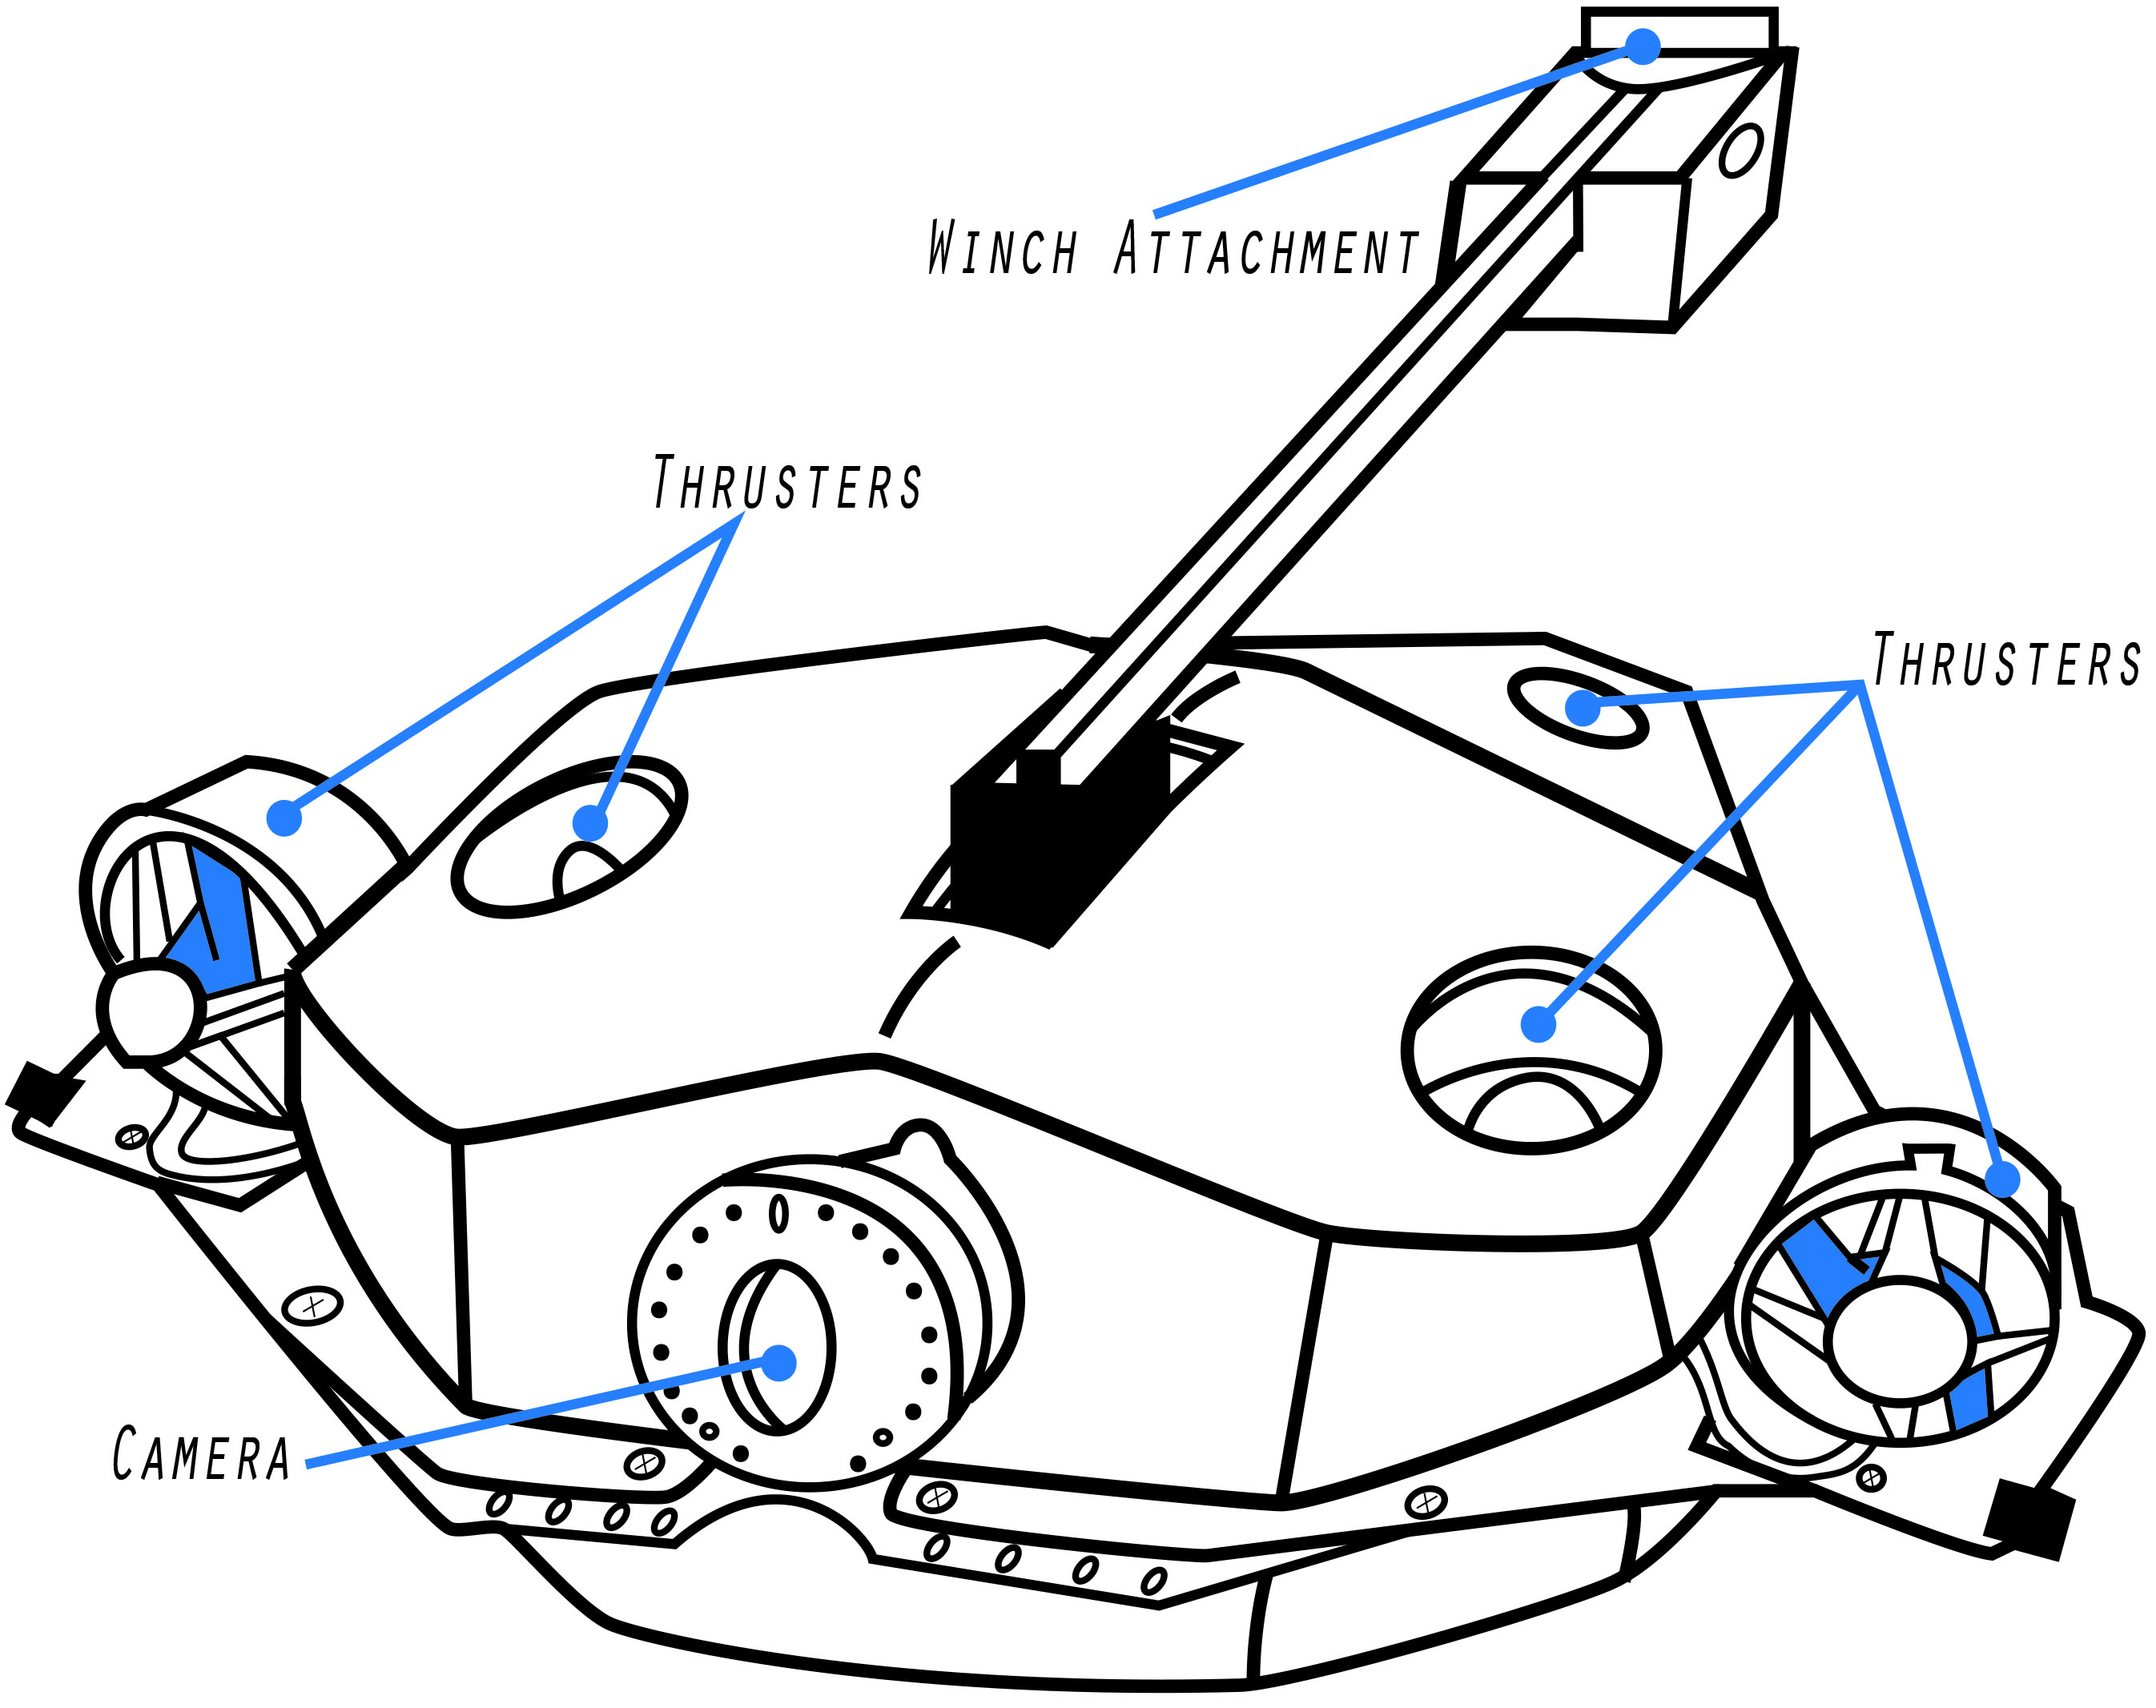
\includegraphics[width=0.9\linewidth]{Figures/Component_Diagrams/basic_sub.jpg}
	\caption[]{An overview of the submarine} % The text in the square bracket is the caption for the list of figures while the text in the curly brackets is the figure caption 
\end{figure}
\begin{figure}[H]
	\centering 
	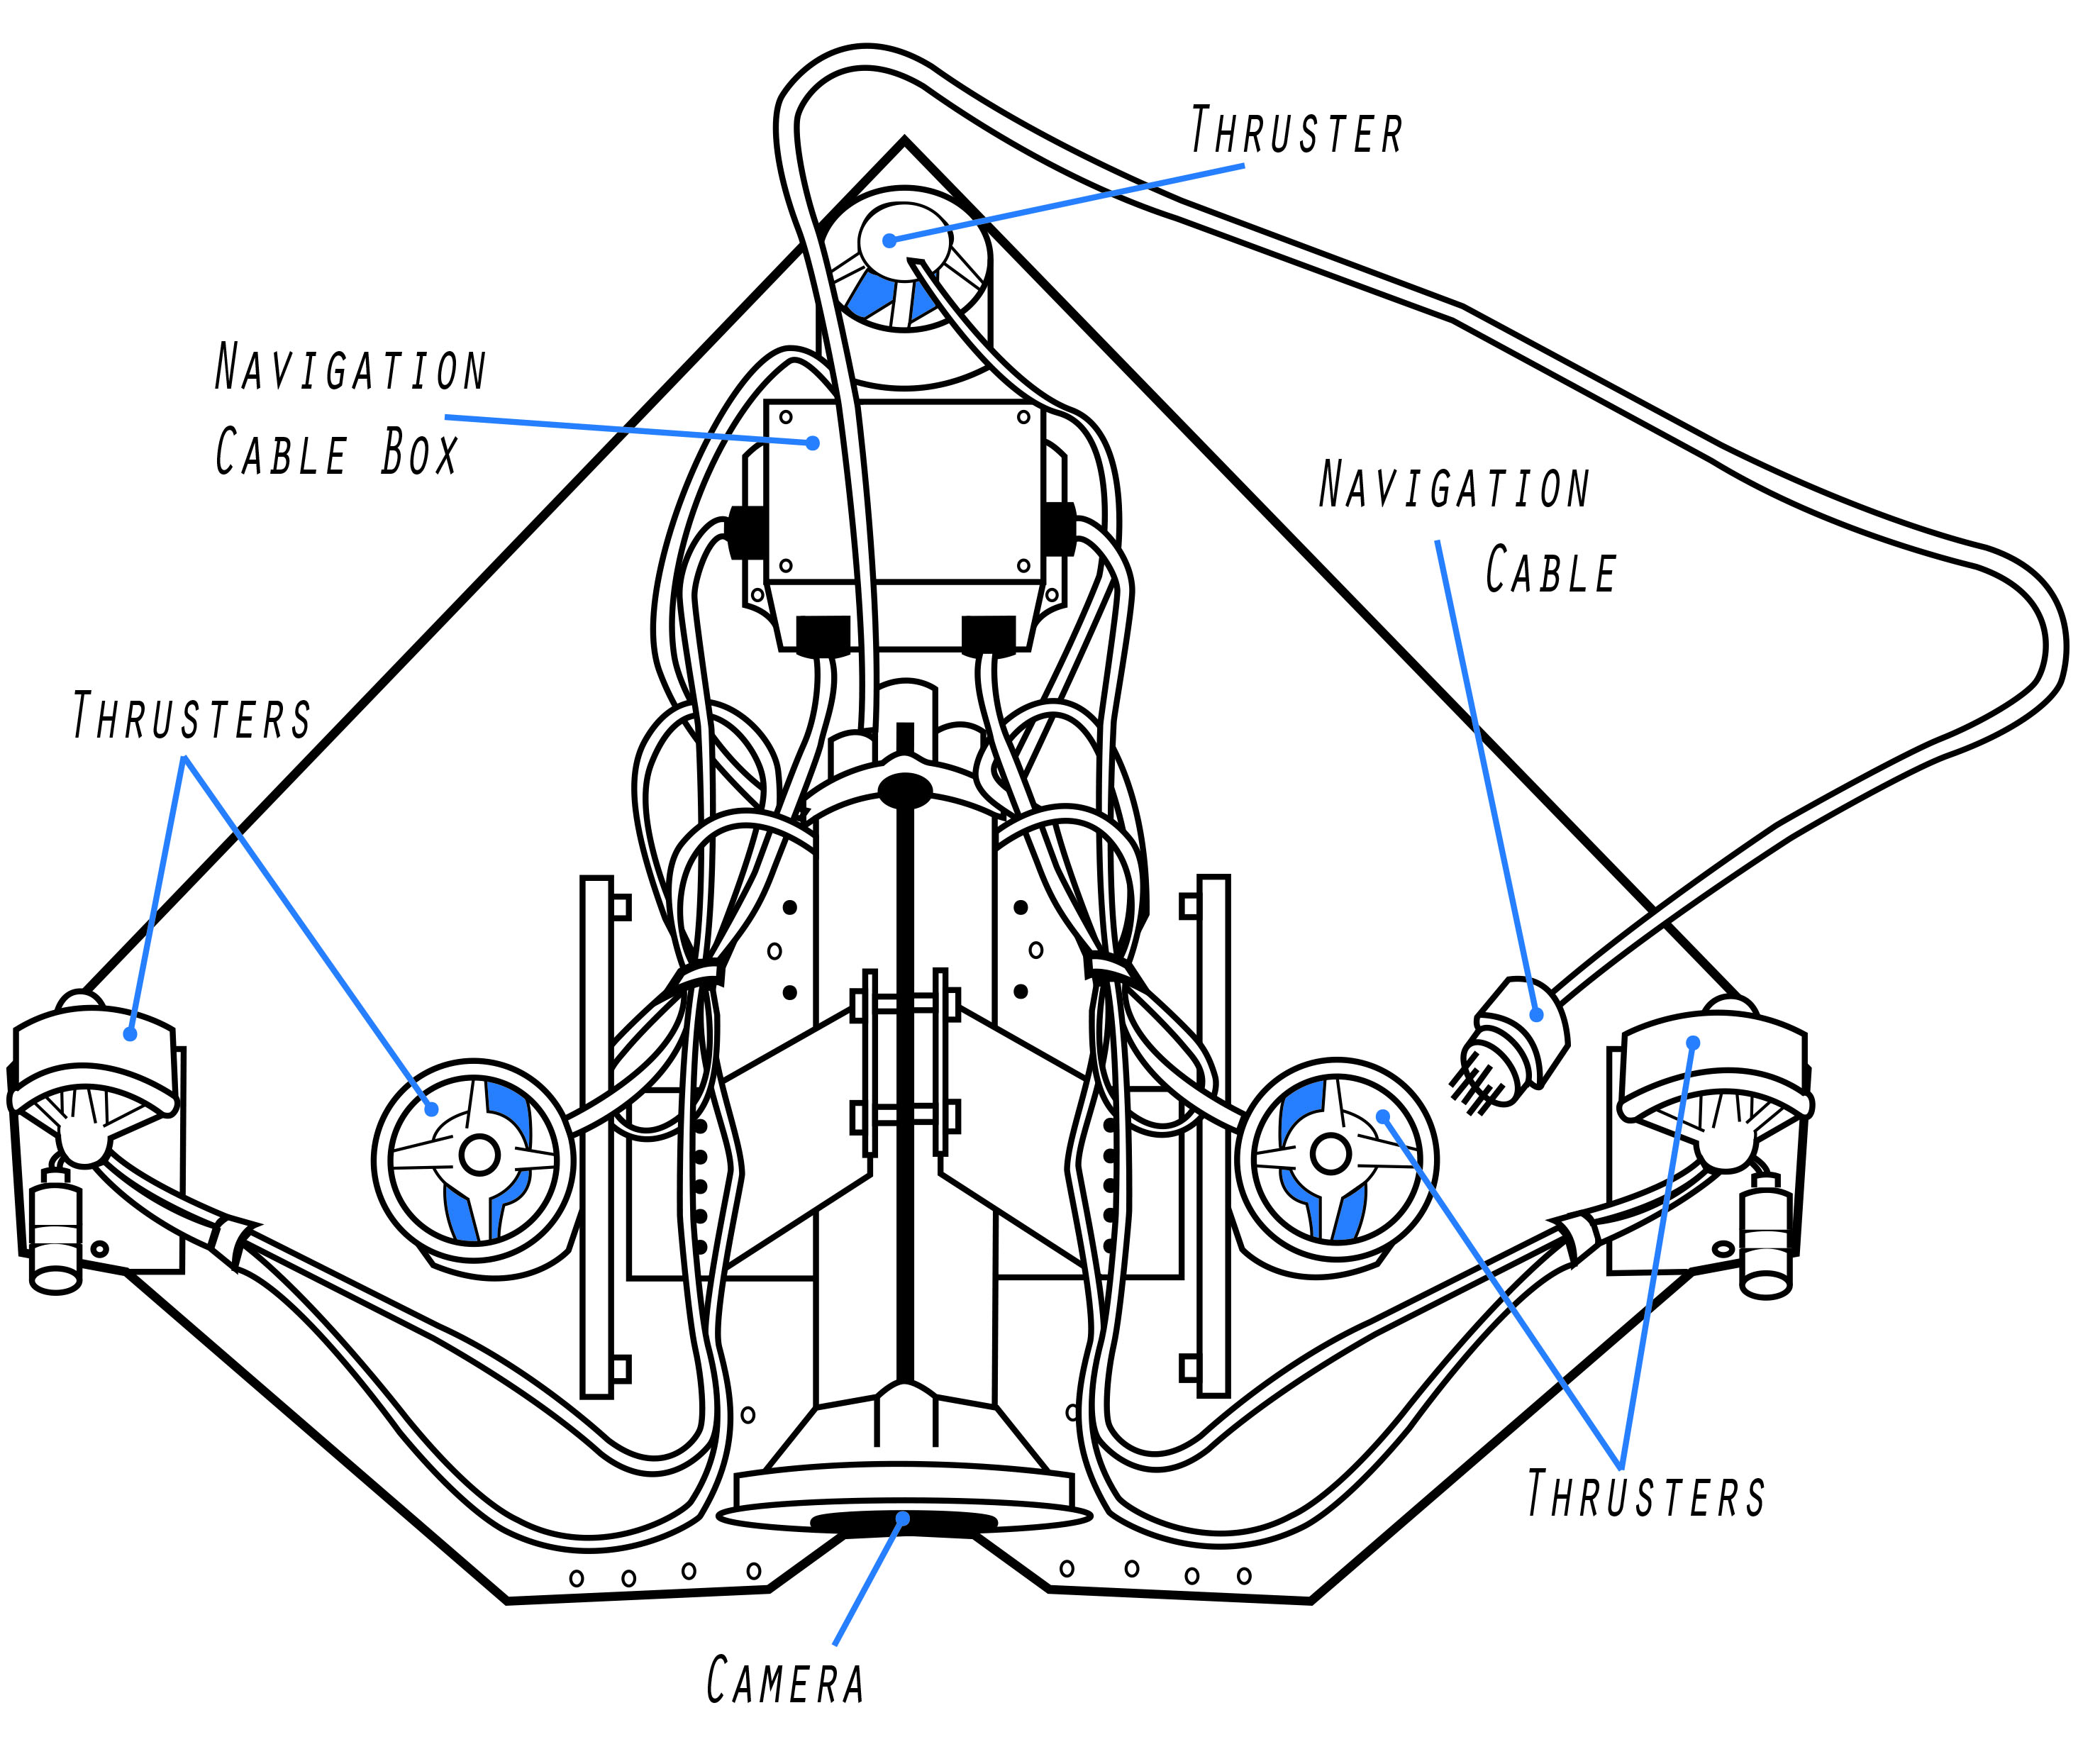
\includegraphics[width=0.9\columnwidth]{Figures/Component_Diagrams/inside_sub.jpg}
	\caption[]{An inside view of the submarine} % The text in the square bracket is the caption for the list of figures while the text in the curly brackets is the figure caption 
\end{figure}
\begin{figure}[H]
	\centering 
	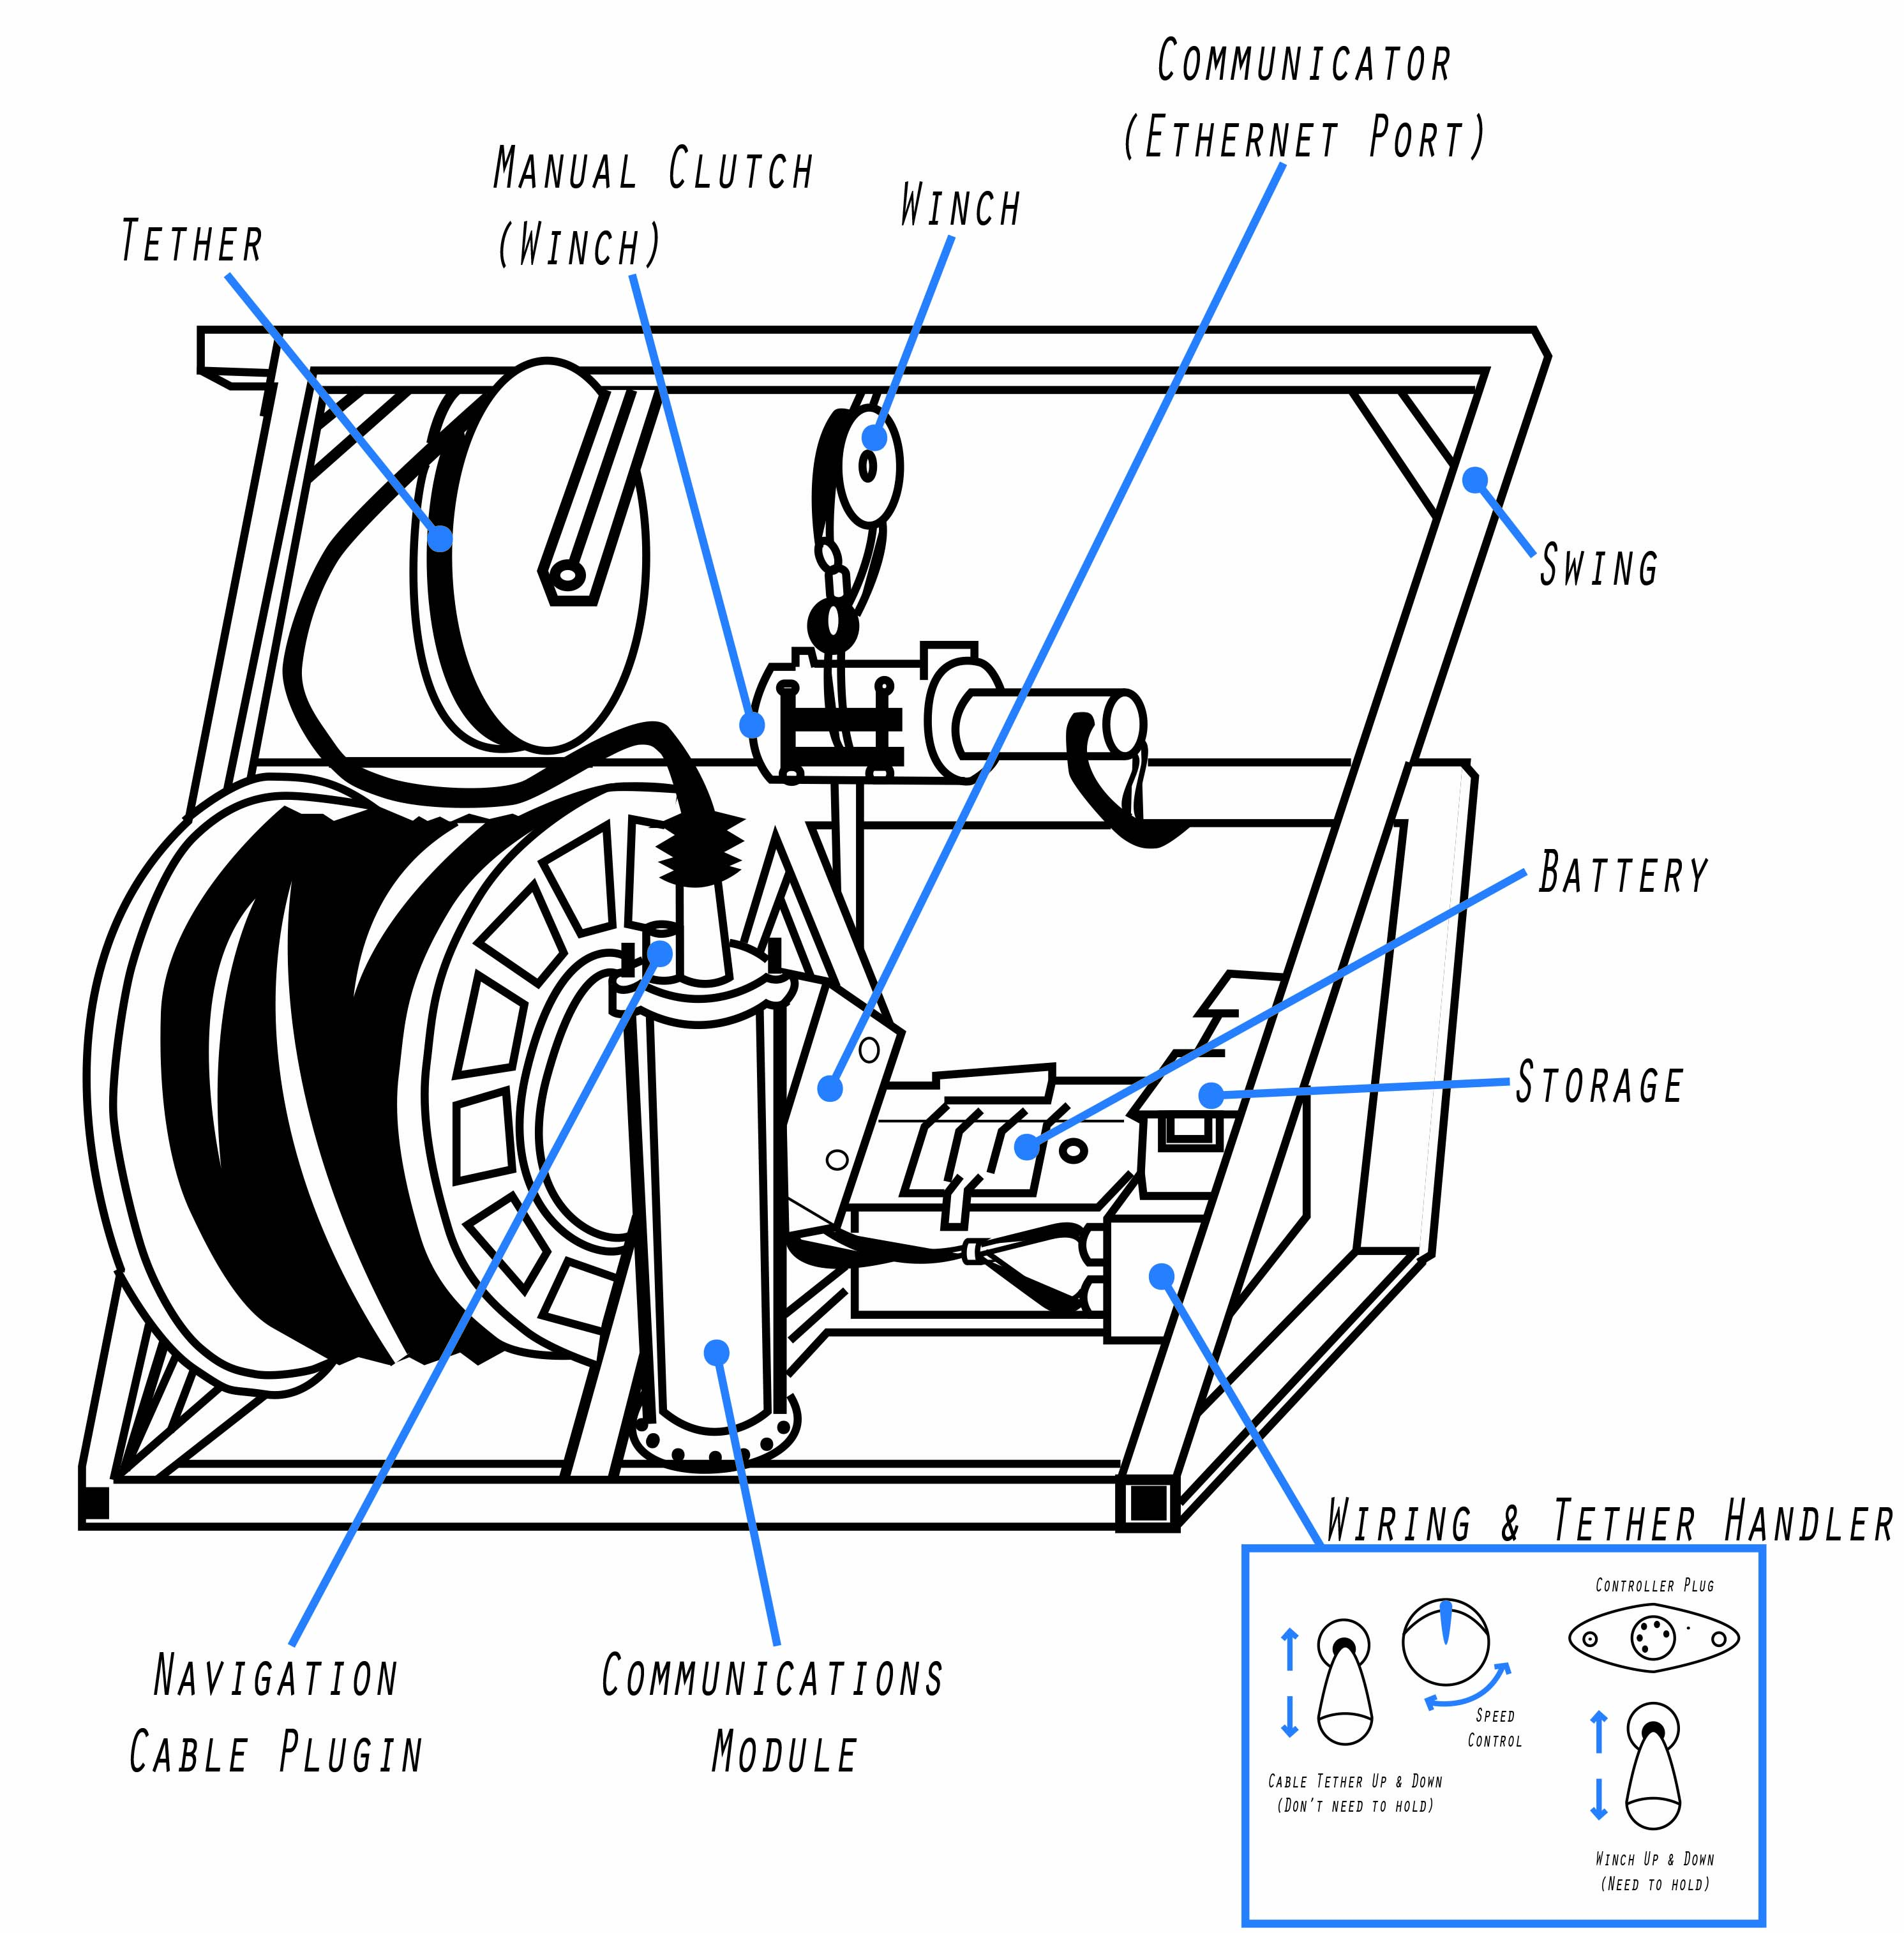
\includegraphics[width=0.9\columnwidth]{Figures/Component_Diagrams/handling_gear.jpg}
	\caption[]{An overview of the handling gear} % The text in the square bracket is the caption for the list of figures while the text in the curly brackets is the figure caption 
\end{figure}
\begin{figure}[H]
	\centering 
	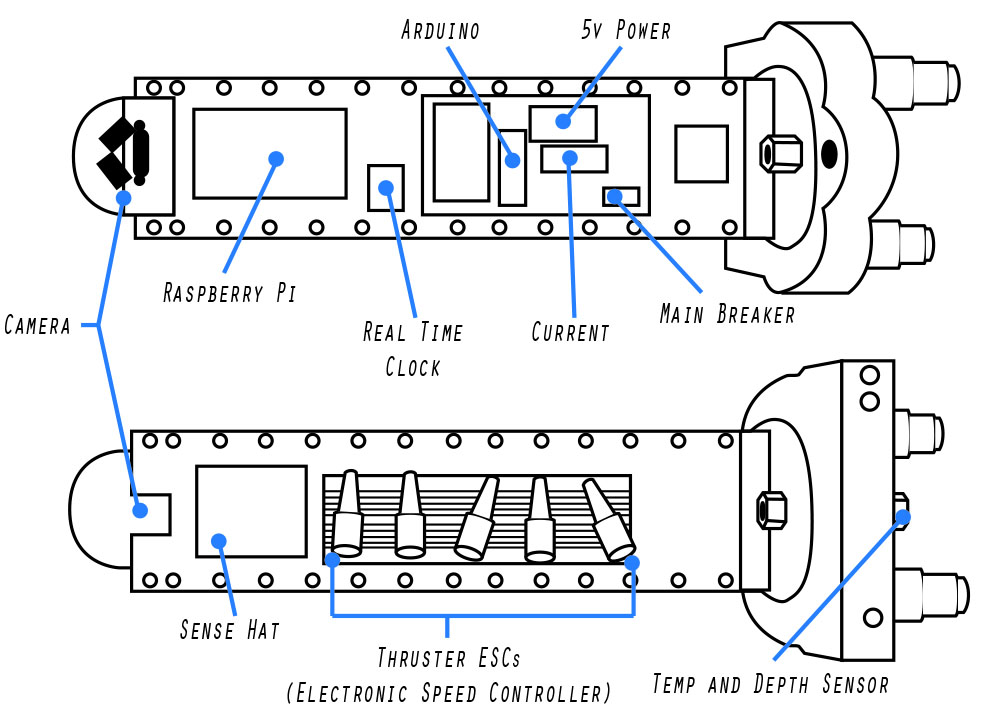
\includegraphics[width=0.9\columnwidth]{Figures/Component_Diagrams/navigation_board.jpg}
	\caption[]{An inside view of the communications module} % The text in the square bracket is the caption for the list of figures while the text in the curly brackets is the figure caption 
\end{figure}
\clearpage
\newpage
%------------------------------------------------

\subsection{Power on/off}

Located on the back of the submarine is a power station with plugs. Each plug is labeled: PI, PWR, GRND. These are acronyms. PI stands for Raspberry Pi, it has its' own battery contained in the submarine. PWR runs to two separate batteries that have been linked together. Both batteries power the thrusters of the submarine. This is because the thrusters take so much power, by giving them two batteries, they last longer; also by separating them from the Raspberry Pi, if one dies it doesn't affect the integrity of the other. GRND stands for ground, its sole purpose is merely for charging the batteries.

%------------------------------------------------

\subsection{Charging Battery}

There are two separate chargers for charging the batteries as well as two separate sets of batteries. One set of batteries is inside the submarine, and the other set is on the handling gear.

\paragraph{The Charger}
The charger itself has an indicator on the back. By attaching the required charger to the battery it will tell you how much power is remaining as well as the charging progress. The charger also has a trickle feature, so it can be left plugged in overnight and will not overcharge the battery.\\ \\
There is also a charge indicator provided as a separate device. When measuring the charge, it is in voltage not percent. The nominal charge is 12V, fully charged is 13V, and low voltage is 11V. \\ \\
DO NOT let the batteries get below 11V. It is NOT recommended.

\paragraph{Submarine Battery Charge}
When charging the submarine, you can only charge one of the battery sets inside at a time. This is because of the way the charger was designed. So either the Raspberry Pi or the thrusters can be charged. \\ \\
In order to begin charging, the red attachment will be plugged into the desired battery port and the black attachment will always be plugged into ground. Charging the submarine (both battery sets) will take about 12 hours. It is recommended to charge the submarine after each deployment.

\paragraph{Handling Gear Charge}
When charging the handling gear, it functions in much the same way as the submarine. You will attach the charger to the handling gear battery, red to power and black to ground. Testing the handling gear battery charge is recommended but it lasts a very long period of time so frequent charges are not required.

%------------------------------------------------

\subsection{Deployment}

TO BE FILLED IN WITH ADRIAN'S ASSISTANCE, DUMMY TEXT FOLLOWS

\lipsum[6]

%------------------------------------------------

%------------------------------------------------

\subsection{Checks}

The purpose of these checks is to ensure the functionality of all submarine and handling gear parts both before and after deployment.

\paragraph{Handling Gear - Preoperational Checks} Before operating the handling gear, it is important to go through the following checks:

\begin{itemize}[noitemsep] % [noitemsep] removes whitespace between the items for a compact look
	\item Voltage check
	\item Winch check
	\item Reel check
	
\end{itemize}
Further descriptions of the aforementioned checks are as follows:

\begin{description}
	\item[Voltage Check] In order to check the voltage of the handling gear battery, merely use the provided voltage check device in the same manner as the battery charger. Attach the red wire to power and the black wire to ground. The handling gear battery is very long lasting and therefore this check does not need to be done after every deployment, but also should not be significantly deferred.
	\item[Winch Check] In order to make sure the winch wire itself isn't caught or in any way impeded, merely release the manual winch switch and pull on the wire. Then, in order to rest the integrity of power raising/lowering of the wire, use the control box on the side of the handling gear. Make sure to test both the forward and reverse aspects of the winch. 
	\item[Reel Check] The reel check is merely testing the large tether and making sure it has free movement and connection. The fiber-optic cable should be free to move, both in forward and reverse. There is a switch respective to this on the control box of the handling gear.
\end{description}

\paragraph{Submarine - Preoperational Checks} In order to ensure the integrity of the submarine hull prior to a deployment, the following checks should be conducted:

\begin{itemize}[noitemsep] % [noitemsep] removes whitespace between the items for a compact look
	\item Control module all thread torque checked
	\item Vertical thruster mount bolts checked
	\item Thruster to control module cables and connectors checked
	\item Light to control module cables and connectors checked
	\item Syntactic foam intact
	\item Other cables to control module?
	\item Mast attachment bolt torque checked
\end{itemize}

Further descriptions of the aforementioned checks are as follows:

\begin{description}
	\item[Control Module Thread Torque] \lipsum[7] % Dummy text
	\item[Vertical Thruster Mount Bolts] \lipsum[7] % Dummy text
	\item[Thruster to Control Module Cables and Connectors] \lipsum[7] % Dummy text
	\item[Light to Control Module Cables and Connectors] \lipsum[7] % Dummy text
	\item[Syntatic Foam] \lipsum[7] % Dummy text
	\item[Other Cables to Control Module?] \lipsum[7] % Dummy text
	\item[Mast Attachment Bolt Torque] \lipsum[7] % Dummy text
\end{description}

\paragraph{Submarine - Postoperational Checks} \lipsum[7] % Dummy text

\begin{itemize}[noitemsep] % [noitemsep] removes whitespace between the items for a compact look
	\item Voltage check
	\item Physical check
	\item All shell bolts in-place and torque checked
	\item Vehicle to Communication module cable connected
	\item Final ballast system accessible
\end{itemize}

Further descriptions of the aforementioned checks are as follows:

\begin{description}
	\item[Voltage check] \lipsum[7] % Dummy text
	\item[Physical check] \lipsum[7] % Dummy text
	\item[All shell bolts in-place and torque checked] \lipsum[7] % Dummy text
	\item[Vehicle to Communication module cable connected] \lipsum[7] % Dummy text
	\item[Final ballast system accessible] \lipsum[7] % Dummy text
\end{description}
%------------------------------------------------

%----------------------------------------------------------------------------------------
%	USING SOFTWARE
%----------------------------------------------------------------------------------------

\section{Using Software}

%------------------------------------------------

\subsection{Connecting to the Submarine}

\paragraph{Ethernet Connection}
\paragraph{Wireless Connection}
\lipsum[6] % Dummy text


%------------------------------------------------
%------------------------------------------------

\subsection{Moving the Submarine}

\lipsum[6] % Dummy text


%------------------------------------------------

%------------------------------------------------

\subsection{Taking Pics/Video}

\lipsum[6] % Dummy text

\paragraph{Where to Save} \lipsum[7] % Dummy text

\paragraph{Streaming} \lipsum[8] % Dummy text

%------------------------------------------------

%----------------------------------------------------------------------------------------
%	SYSTEM CONFIG
%----------------------------------------------------------------------------------------

\section{System Configuration}

\lipsum[10] % Dummy text

%------------------------------------------------

\subsection{Configuring 3D map?}

\lipsum[11] % Dummy text

\subsubsection{Testing with the Turtle}

\lipsum[12] % Dummy text

\lipsum[12] % Dummy text

\subsubsection{Mapping Underwater}

\lipsum[13] % Dummy text


%------------------------------------------------

\subsection{Changing the Raspberry Pi IP's}

\lipsum[15-18] % Dummy text


--------------------------------
%	CONSUMER INFO
%----------------------------------------------------------------------------------------

\section{Consumer Info}

\subsection{Troubleshooting}
\lipsum[5] % Dummy text


\end{document}